\documentclass[12pt]{article}


\usepackage{amssymb}
\usepackage{amsmath}
\usepackage{fullpage}
\usepackage{epsfig}
\usepackage{epstopdf, xcolor, hyperref}
\everymath{\displaystyle}
\usepackage{enumerate}



\begin{document}

\begin{center}
\underline{\LARGE{Double Integrals in Polar Coordinates}}
\end{center}

\noindent SUGGESTED REFERENCE MATERIAL:

\bigskip

\noindent As you work through the problems listed below, you should reference Chapter 14.3 of the recommended textbook (or the equivalent chapter in your alternative textbook/online resource) and your lecture notes.

\bigskip

\noindent EXPECTED SKILLS:

\begin{itemize}

\item Be able to convert rectangular double integrals to polar double integrals, including converting the limits of integration, the function to be integrated, and the differential $dA$ to $r\,dr\,d\theta$.

\end{itemize}

\noindent PRACTICE PROBLEMS:

\medskip

\begin{enumerate}

\item Consider the region $R$ shown below which is enclosed by $x^2+y^2=1$, $x^2+y^2=4$, $y=x$ and the $x$ axis.

\begin{center}
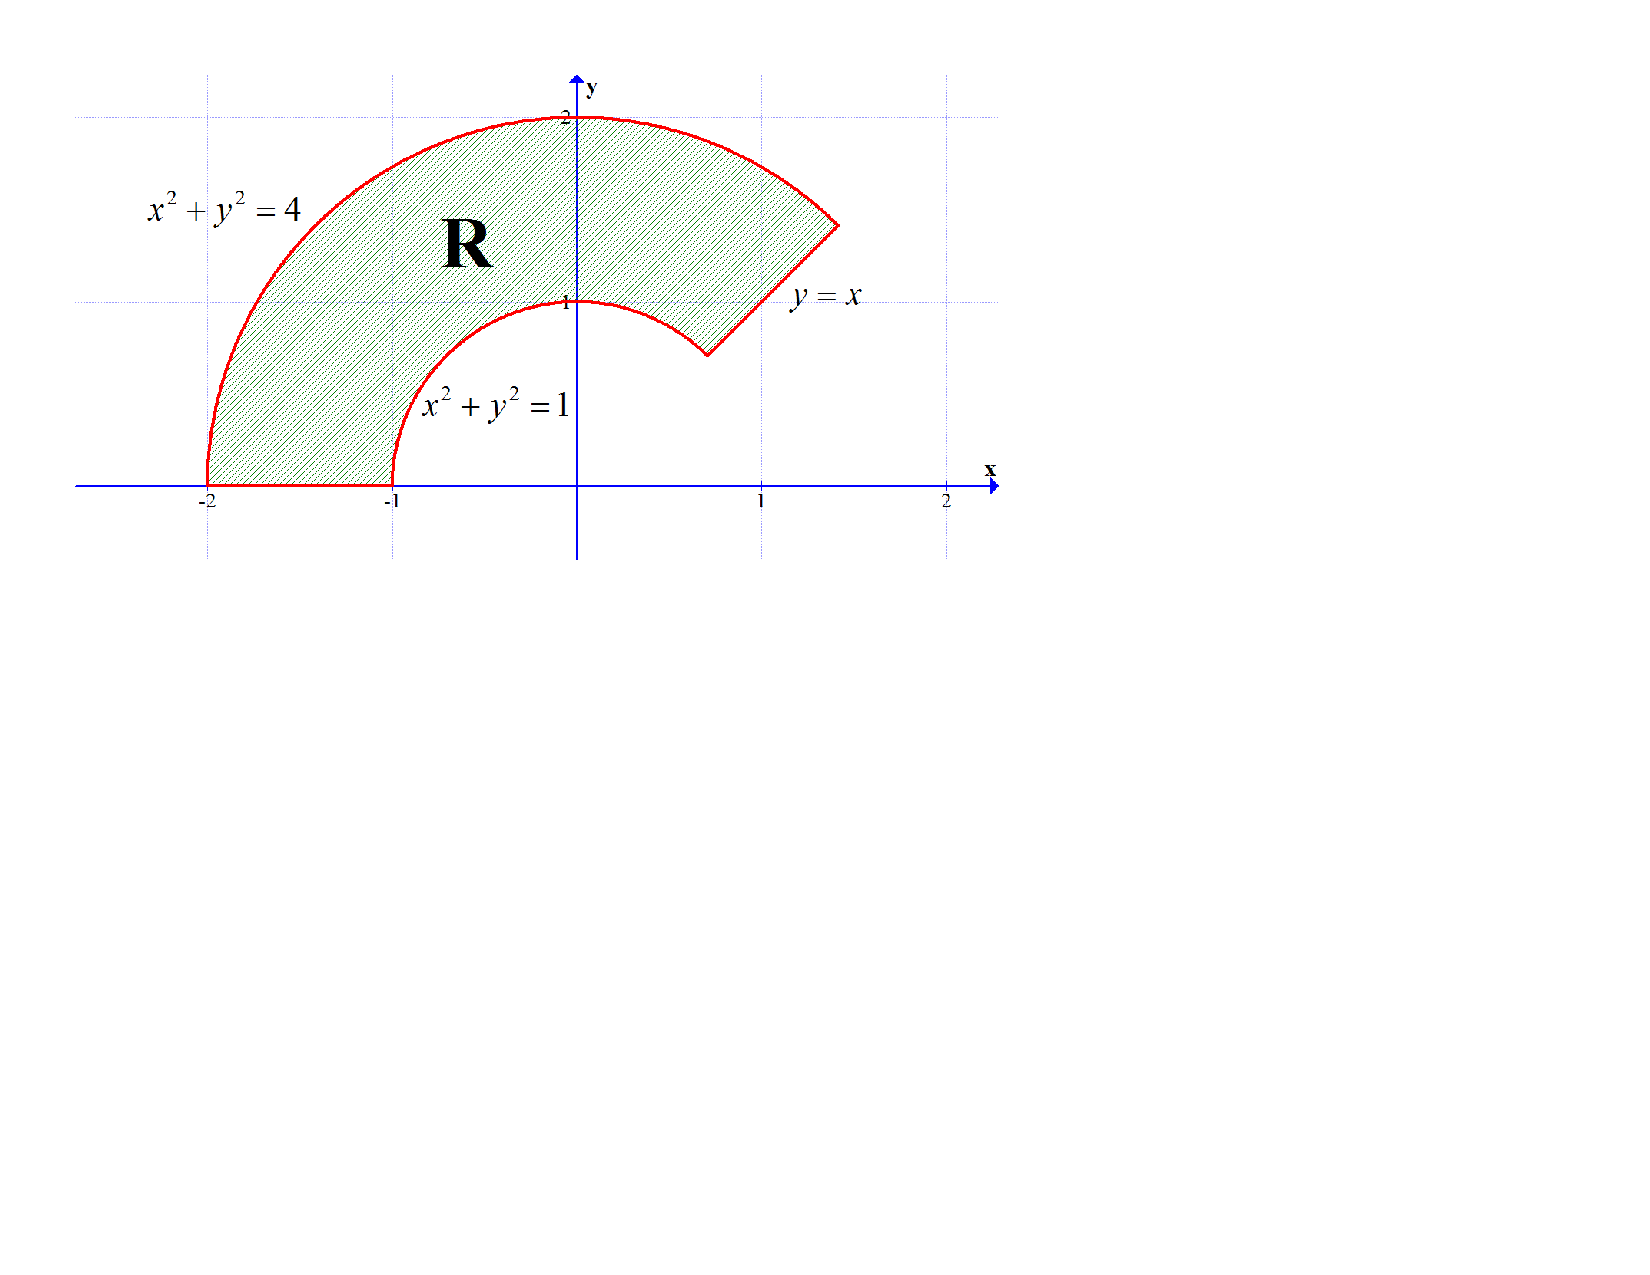
\includegraphics[scale=0.5]{region1.pdf}
\end{center}

Fill in the missing limits of integration: $\iint \limits_{R} f(x,y) \,dA = \int_{\fbox{}}^{\fbox{}}\int_{\fbox{}}^{\fbox{}} f(r,\theta) r \,dr \,d\theta$.

\includegraphics[scale=0.5]{start.pdf}
{{$\iint \limits_{R} f(x,y) \,dA = \int_{\pi/4}^{\pi}\int_{1}^{2} f(r,\theta) r \,dr \,d\theta$}}
\includegraphics[scale=0.5]{end.pdf}


\end{enumerate}

\noindent {\bf For problems 2-6, evaluate the iterated integral by converting to polar coordinates.}

\begin{enumerate}
\setcounter{enumi}{1}

\item $\int_0^{4} \int_0^{\sqrt{16-x^2}} \sqrt{x^2+y^2} \,dy \,dx$

\includegraphics[scale=0.5]{start.pdf}
{{$\frac{32\pi}{3}$}}
\includegraphics[scale=0.5]{end.pdf}


\item $\int_0^{3/\sqrt{2}} \int_x^{\sqrt{9-x^2}} \left(x^2+y^2\right)^2 \,dy \,dx$

\includegraphics[scale=0.5]{start.pdf}
{{$\frac{243}{8}\pi$}}
\includegraphics[scale=0.5]{end.pdf}


\item $\int_0^{2} \int_0^{\sqrt{2x-x^2}} xy \,dy \,dx$

\includegraphics[scale=0.5]{start.pdf}
{{$\frac{2}{3}$}}
\includegraphics[scale=0.5]{end.pdf}


\item Evaluate $\iint \limits_{R} (x-y) \,dA$ where $R=\{(x,y): 4 \leq x^2+y^2 \leq 16 \text{ and } y \leq x\}$

\includegraphics[scale=0.5]{start.pdf}
{{$\frac{112}{3}\sqrt{2}$}}
\includegraphics[scale=0.5]{end.pdf}


\item Evaluate $\iint \limits_{R} e^{-(x^2+y^2)} \,dA$ where $R=\{(x,y): x^2+y^2 \leq 3 \text{ and } 0 \leq y \leq \sqrt{3}x\}$

\includegraphics[scale=0.5]{start.pdf}
{{$\frac{\pi}{6}\left(1-\frac{1}{e^3}\right)$}}
\includegraphics[scale=0.5]{end.pdf}


\item Use a double integral in polar coordinates to calculate the area of the region which is inside of the cardioid $r=2+2\cos{\theta}$ and outside of the circle $r=3$.

\includegraphics[scale=0.5]{start.pdf}
{{$\frac{9\sqrt{3}}{2}-\pi$}}
\includegraphics[scale=0.5]{end.pdf}


\item Use a double integral in polar coordinates to calculate the area of the region which is common to both circles $r=3\sin{\theta}$ and $r=\sqrt{3}\cos{\theta}$.

\includegraphics[scale=0.5]{start.pdf}
{{$\frac{5\pi}{8}-\frac{3\sqrt{3}}{4}$; Detailed Solution: \textcolor{blue}{\href{http://www.math.drexel.edu/classes/Calculus/resources/Math200HW/Solutions/18_200_DI_Polar_08.pdf}{Here}}}}
\includegraphics[scale=0.5]{end.pdf}


\newpage

\item Consider the top which is bounded above by $z=\sqrt{4-x^2-y^2}$ and bounded below by $z=\sqrt{x^2+y^2}$, as shown below.

\begin{center}
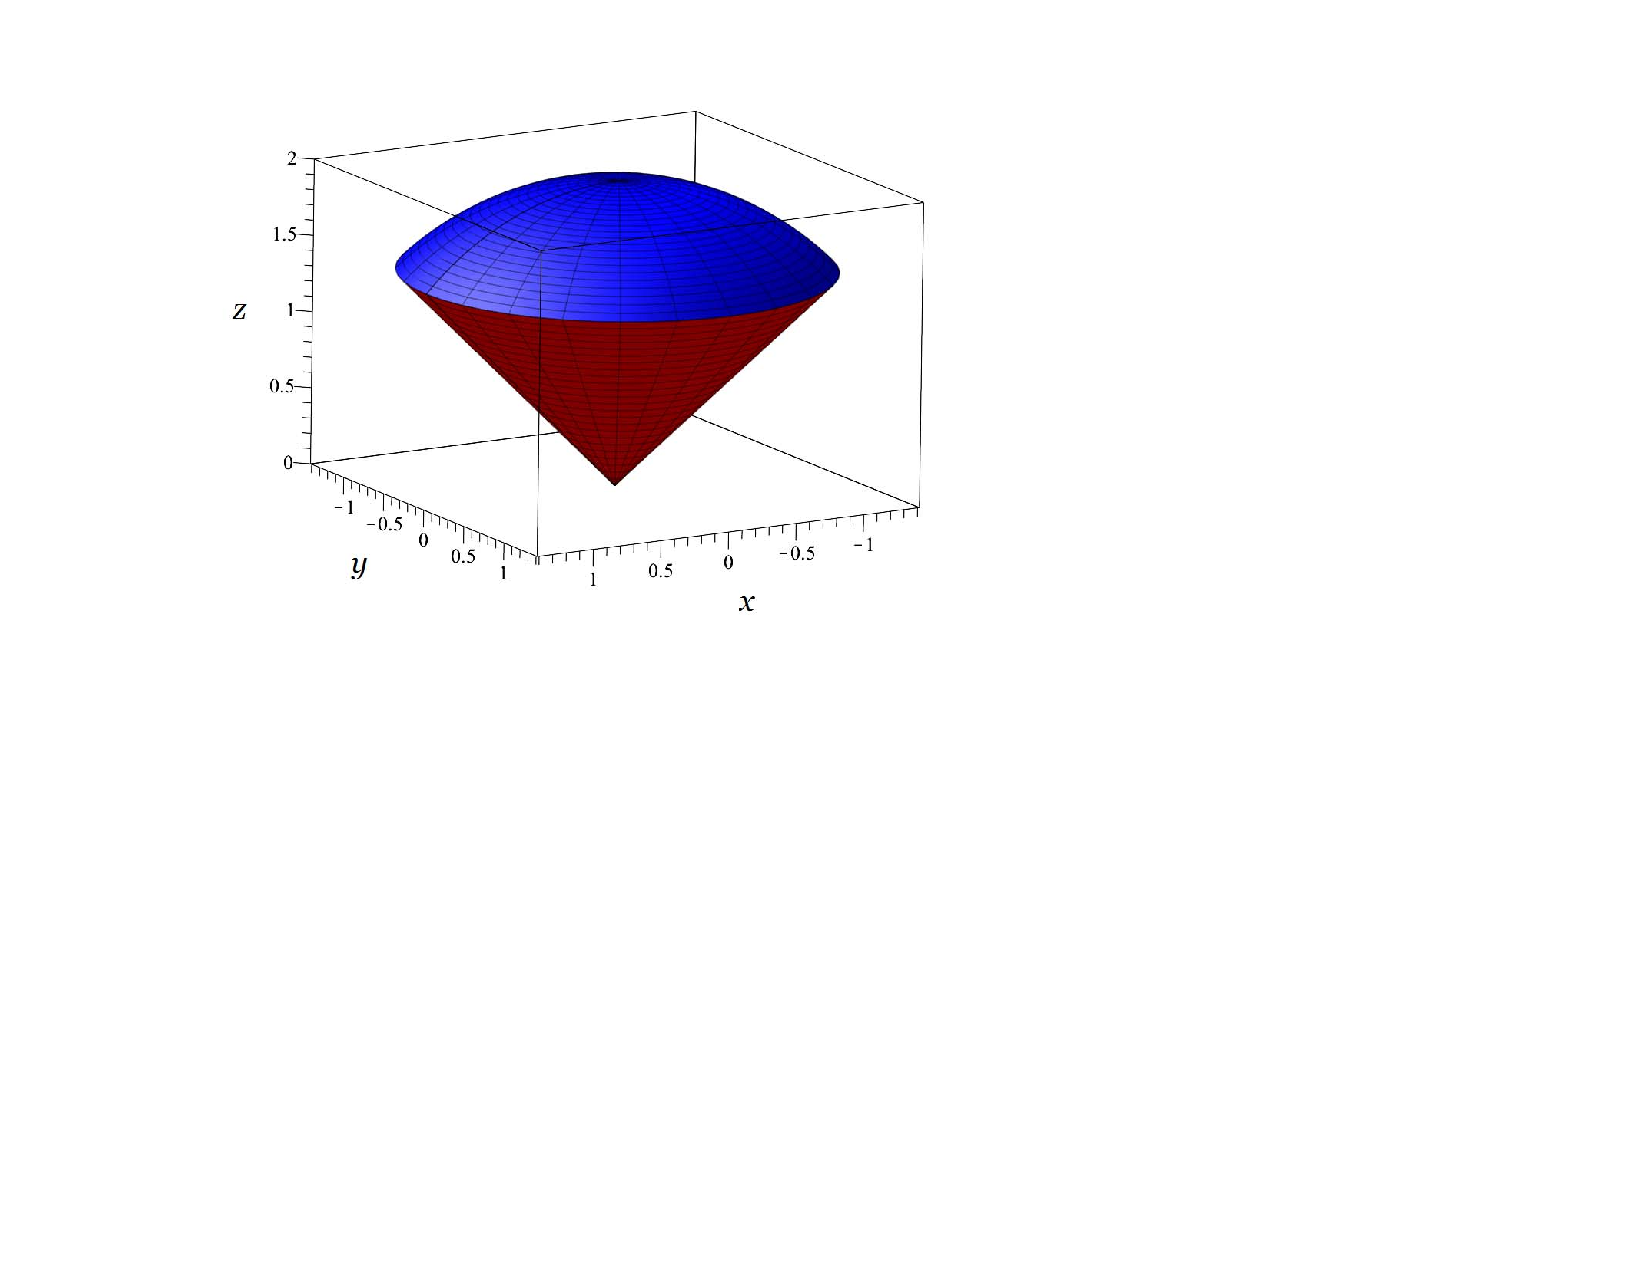
\includegraphics[scale=0.6]{top.pdf}
\end{center}

Use a double integral in polar coordinates to calculate the volume of the top.

\includegraphics[scale=0.5]{start.pdf}
{{$\frac{16\pi}{3}-\frac{8\pi\sqrt{2}}{3}$}}
\includegraphics[scale=0.5]{end.pdf}


\item Consider the surfaces $x^2+y^2+z^2=16$ and $x^2+y^2=4$, shown below.

\begin{center}
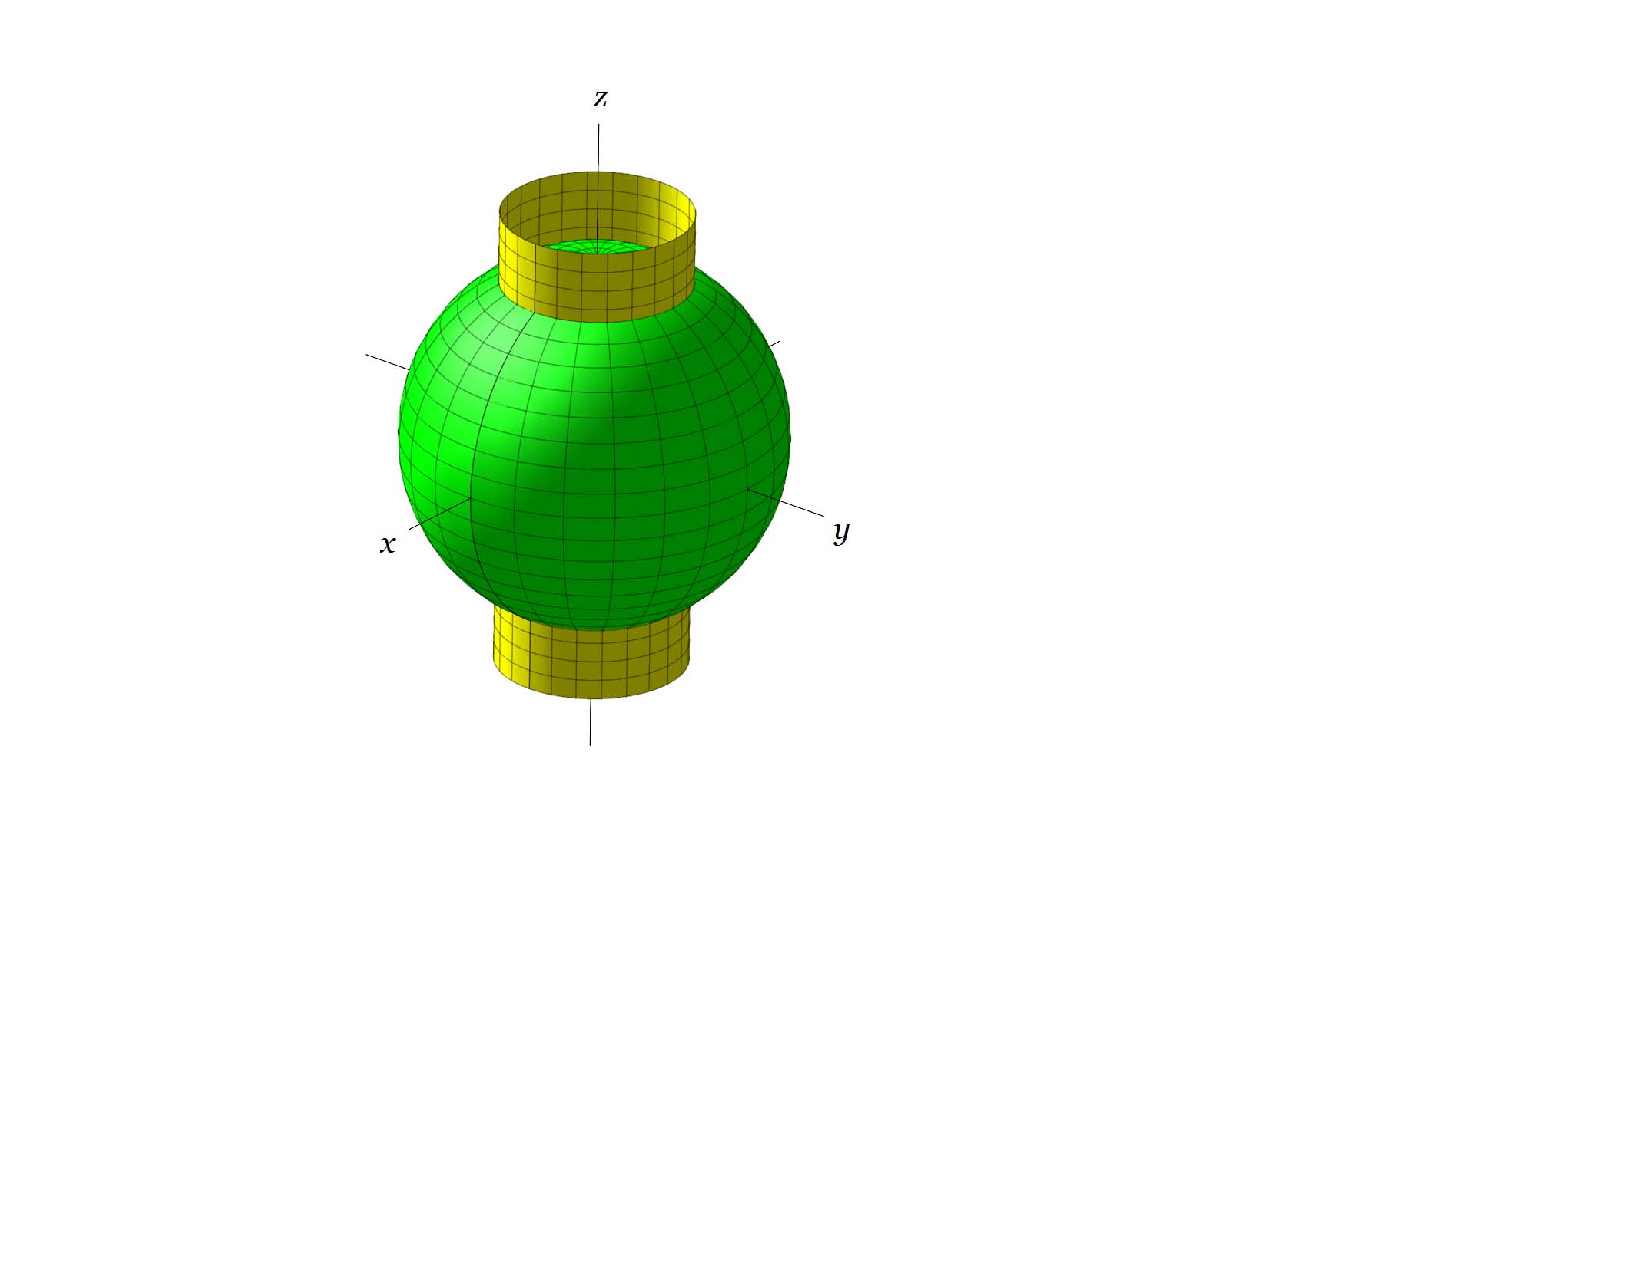
\includegraphics[scale=0.5]{earth.pdf}
\end{center}

Calculate the volume of the solid which is inside of $x^2+y^2+z^2=16$ but outside of $x^2+y^2=4$.

\includegraphics[scale=0.5]{start.pdf}
{{$32\pi\sqrt{3}$; Detailed Solution: \textcolor{blue}{\href{http://www.math.drexel.edu/classes/Calculus/resources/Math200HW/Solutions/18_200_DI_Polar_10.pdf}{Here}}}}
\includegraphics[scale=0.5]{end.pdf}


\newpage

\item Calculate the volume of the solid which is bounded above by $z=9-x^2-y^2$, bounded below by $z=0$, and contained within $x^2-3x+y^2=0$.

\begin{center}
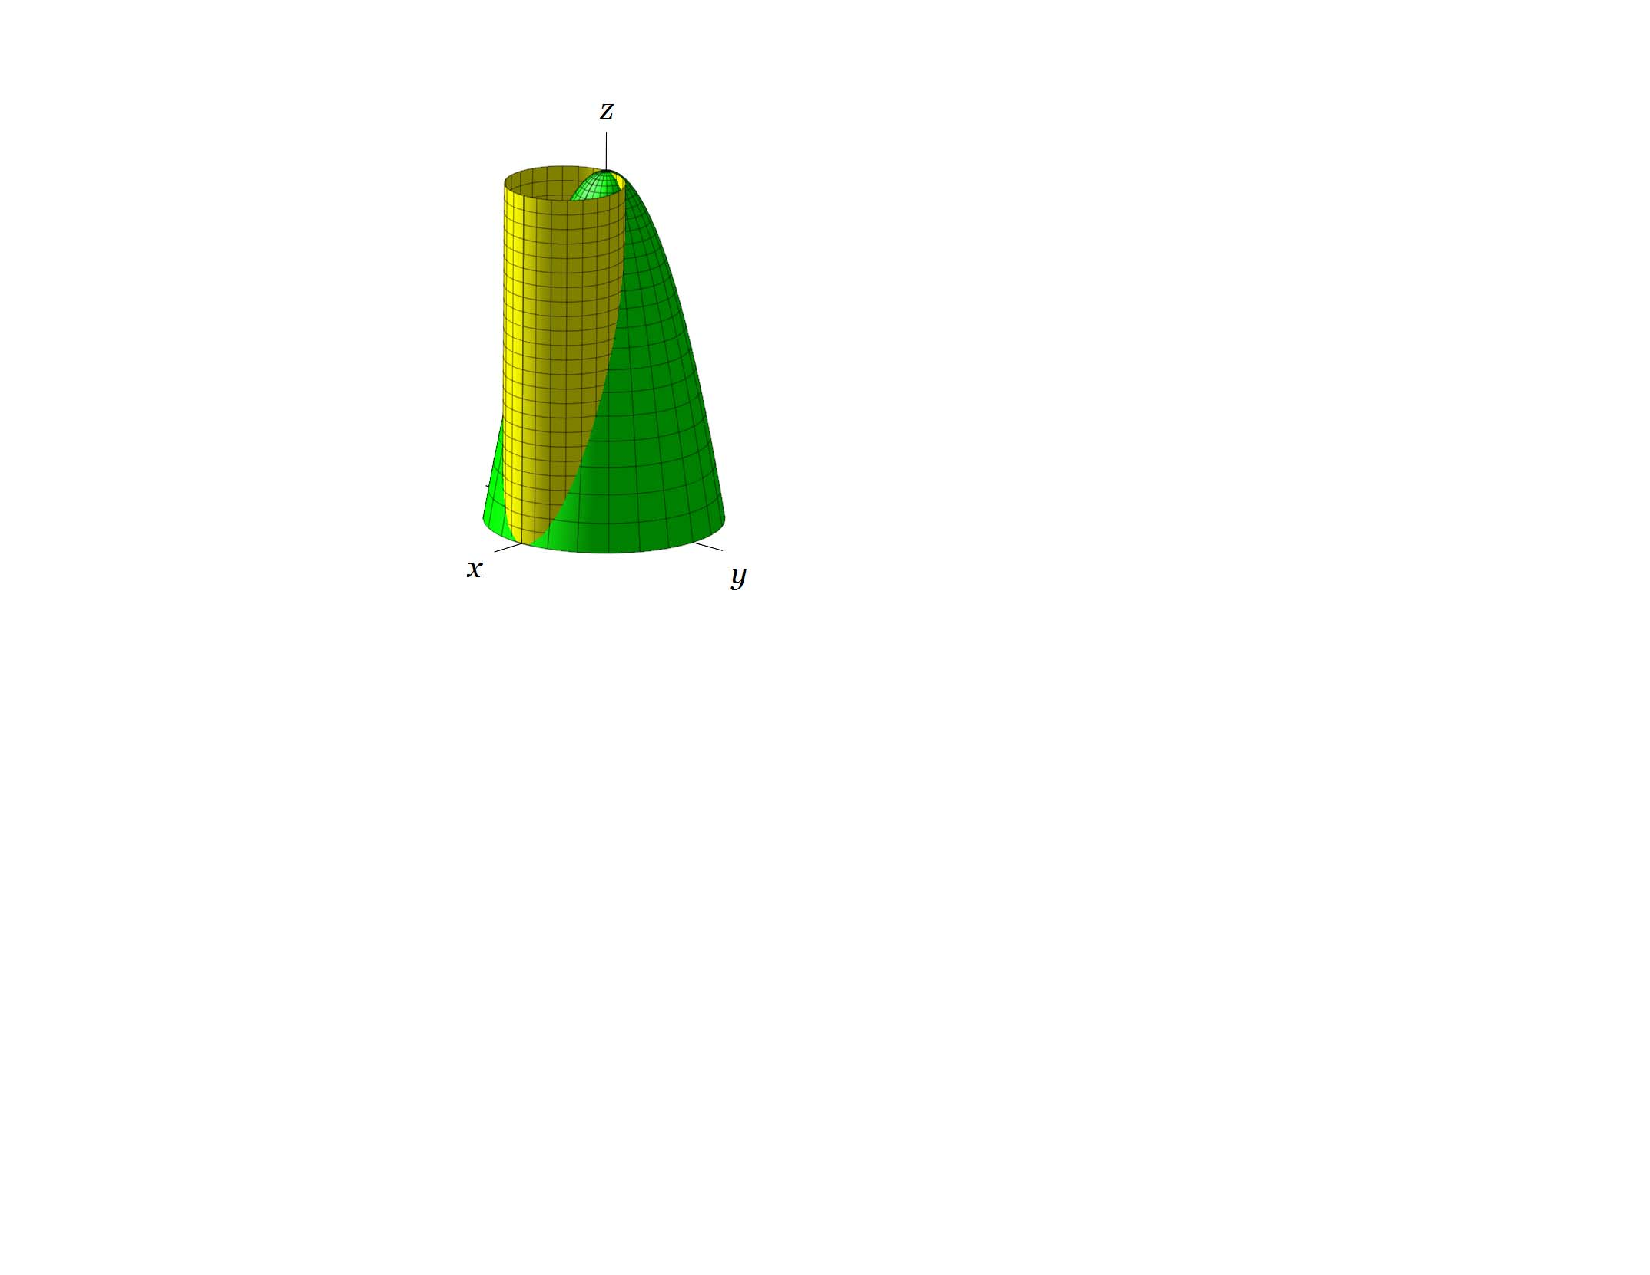
\includegraphics[scale=0.7]{region2.pdf}
\end{center}

\includegraphics[scale=0.5]{start.pdf}
{{$\frac{405\pi}{32}$}}
\includegraphics[scale=0.5]{end.pdf}


\end{enumerate}

\end{document}